\documentclass[12pt,a4paper]{article}
\usepackage{../lecture-notes/vkCourseML}
\usepackage{lipsum}
\usepackage{indentfirst}

\DeclareMathOperator{\Med}{Med}

\title{Машинное обучение, ФКН ВШЭ\\Семинар №6}
\author{}
\date{}
\begin{document}
	\maketitle
	
Грубо говоря, к машинному обучению есть два подхода: инженерный и вероятностный. В предыдущих лекциях мы с вами активно строили функции потерь с помощью инженерного подхода. 

В случае классификации естественно было бы минимизировать долю неправильных ответов, но она недифференцируема. Поэтому мы свели задачу к оптимизации гладкого функционала и придумали несколько верхних оценок. Одной из них была логистическая функция потерь.
	
В случае регрессии мы обсудили среднеквадратичные потери. Оказалось, что они чувствительны к выбросам. Средние абсолютные потери нечувствительны к выбросам, но из-за модуля оптимизировать эту функцию в окрестности оптимума сложнее. Мы скрестили среднеквадратичные потери и абсолютные потери. Получилась функция потерь Хубера.У функции потерь Хубера есть недостаток. Её вторая производная имеет разрывы. Возникла идея придумать гладкую функцию, похожую на функцию Хубера. Так родился Log-Cosh. 

Подобное инженерное мышление помогает придумывать хорошие функции потерь под различные задачи. Иногда можно попробовать поанализировать функции потерь с помощью вероятностного подхода и немного лучше понять, как именно они работают. В этом семинаре мы попытаемся понять, что именно прогнозируют модели, когда мы используем ту или иную функцию потерь. 

\section{Эмпирические и теоретические потери}

Когда мы обучаем модель, мы считаем ошибку на обучающей выборке и минимизируем её по параметрам модели $a(x)$

\[
\frac{1}{\ell} \sum_{i=1}^{\ell} L(y_i, a(x_i)) \to \min_{w}
\]

В зависимости от того, какая выборка оказалась у нас в руках, могут получаться разные оценки параметров модели. При разных обучающих выборках, эмпирические потери могут принимать разные значения при одних и тех же параметрах модели. Эмпирическая функция потерь --- это случайная величина. На самом деле, нам хотелось бы оптимизировать математическое ожидание ошибки

\[
\mathbb{E}(L(y, a(x)) \mid x).
\]

Мы его не знаем, поэтому для его оценки мы используем эмпирические потери. Почему можно это делать? Эмпирические потери --- это выборочное среднее. По закону больших чисел оно должно при больших значениях $\ell$ сходиться к математическому ожиданию.

Ошибка на обучающей выборке $\frac{1}{\ell} \cdot \sum_{i=1}^{\ell} L(y_i, a(x_i))$ --- это эмпирическая оценка ожидаемых потерь $\mathbb{E}(L(y, a(x)) \mid x)$. Этот факт позволяет по-новому взглянуть на старые функции потерь. Минимизируя $\mathbb{E}(L(y, a) \mid x)$ по прогнозам, $a$, можно понять, что именно прогнозирует наш алгоритм. 

Пусть выборка пришла к нам из какого-то распределения. Будем считать, что в каждой точке $x \in \XX$ пространства объектов задано вероятностное распределение~$p(y \cond x)$ на возможных ответах для данного объекта.

Такое распределение может возникать, например, в задаче предсказания кликов по рекламным баннерам:
один и тот же пользователь может много раз заходить на один и тот же сайт и видеть данный баннер;
при этом некоторые посещения закончатся кликом, а некоторые~--- нет.

\section{Что предсказывают модели регрессии}

\begin{vkProblem}
    Пусть для оптимизации мы используем $MSE$, то есть $L(y, a(x)) = (y - a(x))^2.$ Покажите, что оптимальным прогнозом в таком случае будет условное математическое ожидание $\mathbb{E}(y \mid x).$
\end{vkProblem}

\begin{esSolution}
Запишем математическое ожидание потерь

\[
\mathbb{E}\left[L(y, a(x)) \mid x \right] = \mathbb{E} \left[ (y - a(x))^2 \mid x \right] = \int_{-\infty}^{+\infty} (y - a(x))^2  p(y \mid x) dy.
\]

Будем перебирать все возможные значения прогноза $a$ так, чтобы минимизировать математическое ожидание функции потерь

\[
\int_{-\infty}^{+\infty} (y - a)^2  p(y \mid x) dy \to \min_{a}.
\]

Найдём производную по $a$ и приравняем её к нулю

\begin{align*}
    \frac{\partial }{\partial a} \left(  \int_{-\infty}^{+\infty} (y - a)^2 \cdot p(y \mid x) dy  \right) &= - 2 \cdot \int_{-\infty}^{+\infty} (y - a) \cdot p(y \mid x) dy = 0 \\ 
    \int_{-\infty}^{+\infty} y \cdot p(y \mid x) dy  - \int_{-\infty}^{+\infty}  a \cdot p(y \mid x) dy  &= \mathbb{E}(y \mid x) - a \cdot 1 =  0 \Rightarrow  a = \mathbb{E}(y \mid x).
\end{align*}

Получается, что при квадратичных потерях, оптимальным прогнозом будет условное математическое ожидание. Из-за этого алгоритмы, которые обучаются на квадратичные потери, чувствительны к выбросам.  Одно большое значение довольно сильно искажает среднее.
\end{esSolution}
 
Давайте вспомним, как брать производную от интеграла переменным пределами интегрирования

\[
\frac{d}{d \alpha} \int_{a(\alpha)}^{b(\alpha)} f(t, \alpha) dt = \int_{a(\alpha)}^{b(\alpha)} \frac{d f (t, \alpha)}{d \alpha}  dt  + f (b(\alpha), \alpha) \cdot \frac{d b(\alpha)}{d \alpha} - f (a(\alpha), \alpha) \cdot \frac{d a(\alpha)}{d \alpha}.
\]

Производная берётся по $\alpha.$ Пределы интегрирования зависят от  $\alpha.$ Из-за этого возникают два дополнительных слагаемых. В следующих задачах прогноз $a$ бедут присутствовать в пределах интегрирования, но $f(b(\alpha), \alpha) = f(a(\alpha), \alpha) = 0.$
 
\begin{vkProblem}
    Пусть для оптимизации мы используем $MAE$, то есть $L(y, a(x)) = |y - a(x)|.$ Покажите, что оптимальным прогнозом в таком случае будет условная медиана.
\end{vkProblem}

\begin{esSolution}
Запишем ожидаемые потери

\[
\mathbb{E}\left[L(y, a(x)) \mid x \right] = \mathbb{E} \left[ |y - a(x)| \mid x \right] = \int_{-\infty}^{+\infty} |y - a(x)| \cdot p(y \mid x) dy.
\]

Будем перебирать все возможные значения прогноза $a$ так, чтобы минимизировать математическое ожидание функции потерь

\[
\int_{-\infty}^{+\infty} |y - a| \cdot p(y \mid x) dy \to \min_{a}.
\]

Найдём производную по $a$ и приравняем её к нулю. При этом, не будем забывать, что в нуле модуль не дифференцируется. Вероятность того, что непрерывная случайная величина попадёт в конкретную точку, равна нулю. Поэтому мы можем переписать нашу задачу как 

\[
\int_{y > a} (y - a) \cdot p(y \mid x) dy + \int_{y < a} (a - y) \cdot p(y \mid x) dy \to \min_{a}.
\]

Возьмём производную по $a$ и приравняем её к нулю 

\begin{multline*}
\frac{\partial }{\partial a} \left( \int_{y > a} (y - a) \cdot p(y \mid x) dy - \int_{y < a} (a - y) \cdot p(y \mid x) dy  \right) = \\
= \int_{y < a} p(y \mid x) dy - \int_{y > a} p(y \mid x) dy = 0.
\end{multline*}

Получается, что для минимизации ожидаемых потерь надо, чтобы выполнилось равенство $\mathbb{P}(y < a \mid x) = \mathbb{P}(y > a \mid x).$ Точка, в которой выполняется такое равенство, называется медианой. Получается, что $a = \Med(y \mid x)$. 

При абсолютных потерях, оптимальным прогнозом будет условная медиана. Из-за этого алгоритмы, которые обучаются на абсолютные потери, оказываются робастными к выбросам.
\end{esSolution}	    

\section{Квантильная регрессия}

В некоторых задачах цены занижения и завышения прогнозов могут отличаться друг от друга.
Например, при прогнозировании спроса на товары интернет-магазина гораздо опаснее заниженные
предсказания, поскольку они могут привести к потере клиентов.
Завышенные же прогнозы приводят лишь к издержкам на хранение товара на складе.
Функционал в этом случае можно записать как
\[
    Q(a, X^\ell)
    =
    \sum_{i = 1}^{\ell} L(y_i, a(x_i))
        ,
\]
где
\[
    L(y_i, a(x_i)) = \begin{cases} (1 - \alpha) \cdot (a(x_i) - y_i), &a(x_i) > y_i \\  \alpha \cdot ( y_i - a(x_i)), &a(x_i) \le y_i.  \end{cases}
\]


\begin{vkProblem}
    Покажите, что оптимальным прогнозом в таком случае будет условный квантиль уровня $\alpha$.
\end{vkProblem}

\begin{esSolution}

Запишем ожидаемые потери

\[
\mathbb{E}\left[ L(y, a) \mid x \right] = \int_{-\infty}^{a} (1 - \alpha) \cdot (a - y) \cdot  p(y \mid x) dy  + \int_{a}^{+\infty} \alpha \cdot (y - a) \cdot  p(y \mid x) dy \to \min_{a}.
\]

Возьмём производную и приравняем её к нулю 

\[
\frac{\partial \mathbb{E}\left[ L(y, a) \mid x \right]}{\partial a} =  (1 - \alpha) \int_{-\infty}^{a}  p(y \mid x) dy -  \alpha \int_{a}^{+ \infty}  p(y \mid x) dy = 0.
\]

Перепишем это в терминах вероятностей

\[ 
(1 - \alpha) \cdot \mathbb{P}(y \le a \mid x) = \alpha \cdot (1 - \mathbb{P}(y \le \hat y \mid x)).
\]

Решив это уравнение, получаем $\mathbb{P}(y \le a \mid x) = \alpha$. Полученное уравнение --- это определение квантиля уровня $\alpha$. Именно этот квантиль и будет оптимальным прогнозом $a$. 
\end{esSolution}

\section{Предсказание вероятностей}

\par Разберемся, каким требованиям должен удовлетворять классификатор, чтобы его выход можно было расценивать как оценку вероятности класса.

\par Пусть в каждой точке~$x \in \mathbb{X}$ пространства объектов
задана вероятность~$p(y=+1 \cond x)$ того, что данный объект относится
к классу $+1$, и пусть алгоритм~$b(x)$ возвращает числа из отрезка~$[0, 1]$. Потребуем, чтобы эти предсказания пытались в каждой точке~$x$ приблизить вероятность положительного класса~$p(y = +1 | x)$.
\par Разумеется, выполнение этого требования зависит от функции потерь~---
минимум ее матожидания в каждой точке~$x$ должен достигаться на данной вероятности:
$$\arg \min_{b \in \mathbb{R}} \mathbb{E} \left[ L(y, b)|x \right] = p(y=+1|x).$$

\begin{vkProblem}
	Покажите, что квадратичная функция потерь~$L(y, b) = ([y = +1] - b)^2$
	позволяет предсказывать корректные вероятности.
\end{vkProblem}


\begin{esSolution}
	Заметим, что поскольку алгоритм возвращает числа от 0 до 1,
	то его ответ должен быть близок к единице, если объект относится
	к положительному классу, и к нулю~--- если объект относится
	к отрицательному классу.
	
	Запишем матожидание функции потерь в точке~$x$:
	$$\mathbb{E} \left[ L(y, b)|x\right] = p(y=+1|x)(b-1)^2 + (1 - p(y=+1|x))(b-0)^2.$$
	Продифференцируем по~$b$:
	$$\frac{\partial}{\partial b}
	\mathbb{E} \left[
	L(y, b)
	|
	x
	\right] =
	2 p(y = +1 | x) (b - 1)
	+
	2 (1 - p(y = +1 | x)) b
	=
	2b - 2p(y = +1 | x)
	=
	0.$$
	Легко видеть, что оптимальный ответ алгоритма действительно
	равен вероятности:
	$$b = p(y = +1 | x).$$
\end{esSolution}

\begin{vkProblem} Покажите, что абсолютная функция потерь~$L(y, b) = |[y = +1] - b|, \, b \in [0; 1],$
	не позволяет предсказывать корректные вероятности.
\end{vkProblem}
\begin{esSolution}
	Запишем матожидание функции потерь в точке~$x$:
	\begin{align*}
		\mathbb{E} \left[ L(y, b)|x\right] = &p(y=+1|x)|1-b| + (1 - p(y=+1|x))|b| = \\
		&= p(y=+1|x)(1-b)+ (1 - p(y=+1|x))b.\\
	\end{align*}
	Продифференцируем по~$b$:
	$$\frac{\partial}{\partial b}
	\mathbb{E} \left[
	L(y, b)
	|
	x
	\right] =
	1 - 2 p(y = +1 | x) = 0.$$
	Рассмотрим 2 случая:
	\begin{enumerate}
		\item $p(y=+1|x) = \frac{1}{2}.$ Тогда $\mathbb{E} \left[ L(y, b)|x\right] = \frac{1}{2} \quad \forall b \in [0; 1],$ а потому классификатор не позволяет предсказывать корректную вероятность в точке $x$.
		\item $p(y=+1|x) \ne \frac{1}{2}.$ В этом случае интервал $(0; 1)$ не содержит критических точек, а потому минимум матожидания достигается на одном из концов отрезка $[0; 1]:$
		\begin{align*}
			\min_{b \in [0;1]} \mathbb{E} \left[ L(y, b)|x\right] = 
			\min \left(\mathbb{E} \left[ L(y, 0)|x\right], \mathbb{E} \left[ L(y, 1)|x\right] \right) =\\
			\min \left(p(y = +1 | x), 1 - p(y = +1 | x)\right).
		\end{align*}
		Отсюда $\arg \min_{b \in [0;1]} \mathbb{E} \left[ L(y, b)|x\right] \in \{0, 1\},$ а потому классификатор также не позволяет предсказывать корректную вероятность в точке $x$.
	\end{enumerate}
\end{esSolution}

\section{Калибровка вероятностей}

Часто при обучении моделей для бинарной классификации хочется получать не только предсказанную метку класса, но и вероятность положительного класса. Предсказанная вероятность может служить как мера уверенности нашего алгоритма. Однако некоторые алгоритмы не выдают корректные вероятности классов. В таком случае калибруют вероятности модели.

Для начала определимся с тем, что хотим получить от предсказанных вероятностей. В задаче бинарной классификации откалиброванным алгоритмом называют такой алгоритм, для которого доля положительных примеров (на основе реальных меток классов) для предсказаний в окрестности произвольной вероятности $p$ совпадает с этим значением $p$. Например, если взять объекты, для которых предсказанные вероятности близки к 0.7, то окажется, что среди них 70\% принадлежат положительному классу. Для визуализации откалиброванности алгоритма можно построить калибровочную кривую. На этой кривой абсцисса точки соответствуют значению $p$ (предсказаний алгоритма), а ордината соответствует доле положительных примеров, для которых алгоритм предсказал вероятность, близкую к $p$. В идеальном случае эта кривая совпадает с прямой $y = x$. Примеры такой кривой на рис. (\ref{fig:plot}).

\begin{center}
\begin{figure}[!htb]
 \centering
 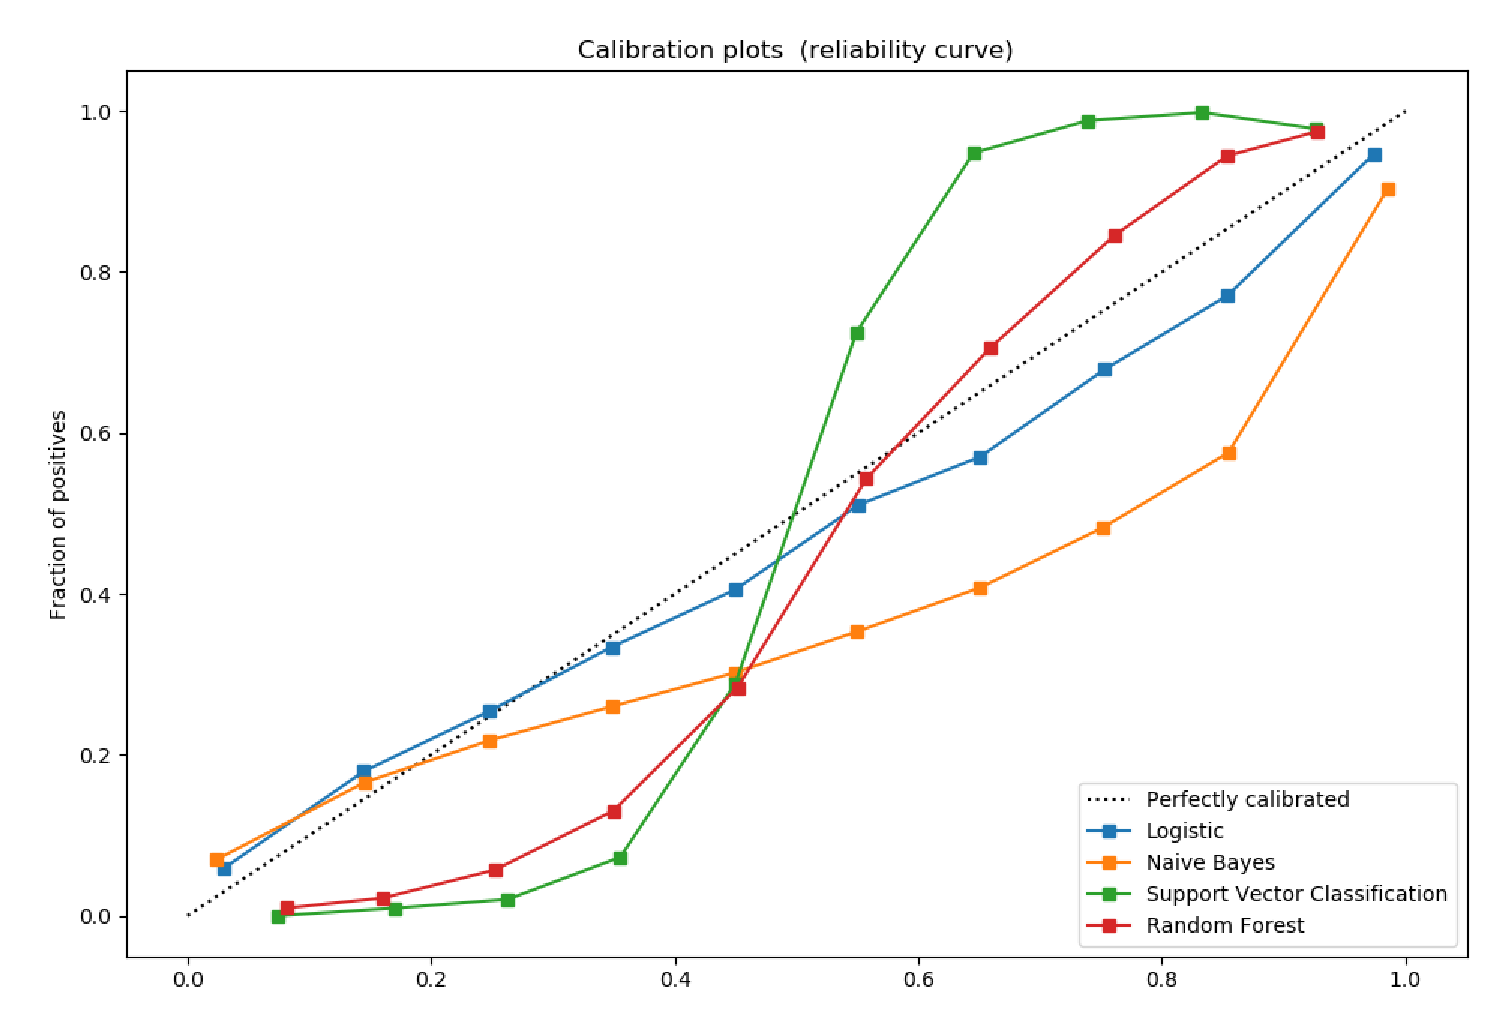
\includegraphics[width=0.7\linewidth]{img/calibration_plot.eps}
 \caption{Калибровочные кривые нескольких алгоритмов}\label{fig:plot}
\end{figure}
\end{center}

Для построения кривой объекты выборки разбиваются на бины $B_m$ по значению предсказанной вероятности, а затем в каждом бине считается доля положительных объектов. В соответствие с кривой можно ввести метрику Expected Calibration Error (ECE), равную усредненному по бинам модулю разности между построенной кривой и прямой $y = x$:

$$
\mathrm{ECE}=\sum_{m=1}^M \frac{\left|B_m\right|}{n}\left|\operatorname{pos}\left(B_m\right)-\operatorname{conf}\left(B_m\right)\right|,
$$

где $\operatorname{pos}(B_m)$ — доля положительных объектов в бине, $\operatorname{conf}(B_m)$ — средняя вероятность положительного класса в бине.

Изучим два стандартных метода для калибровки вероятностей алгоритма: калибровка Платта и изотоническая регрессия.

\subsection{Калибровка Платта}

Пусть наш алгоритм выдаёт значения $f(x)$ (могут не быть вероятностями). Тогда итоговая вероятность:

$$P(y = 1 | x) = \frac{1}{1+\exp (af(x) + b)},$$

где $a, b$ -- скалярные параметры. Эти параметры настраиваются методом максимума правдоподобия (минимизируя логистическую функцию потерь) на отложенной выборке или с помощью кросс валидации. Также Платт предложил настраивать параметры на обучающей выборке базовой модели, а для избежания переобучения изменить метки объектов на следующие значения:

$$t_{+} = \frac{N_{+} + 1}{N_{-} + 2}$$ для положительных примеров и

$$t_{-} = \frac{1}{N_{-} + 2}$$ для отрицательных.

Калибровку Платта можно представить как применения логистической регрессии поверх предсказаний другого алгоритма с отключенной регуляризацией.


\subsection{Изотоническая регрессия}

В этом методе также строится отображение из предсказаний модели в откалиброванные вероятности. Для этого используем изотоническую функцию (неубывающая кусочно-постоянная функция), в которой $x$ -- выходы нашего алгоритма, а $y$ -- целевая переменная. Иллюстрация изотонической регрессии на рис. (\ref{fig:isotonic}).

\begin{center}
\begin{figure}[!htb]
 \centering
 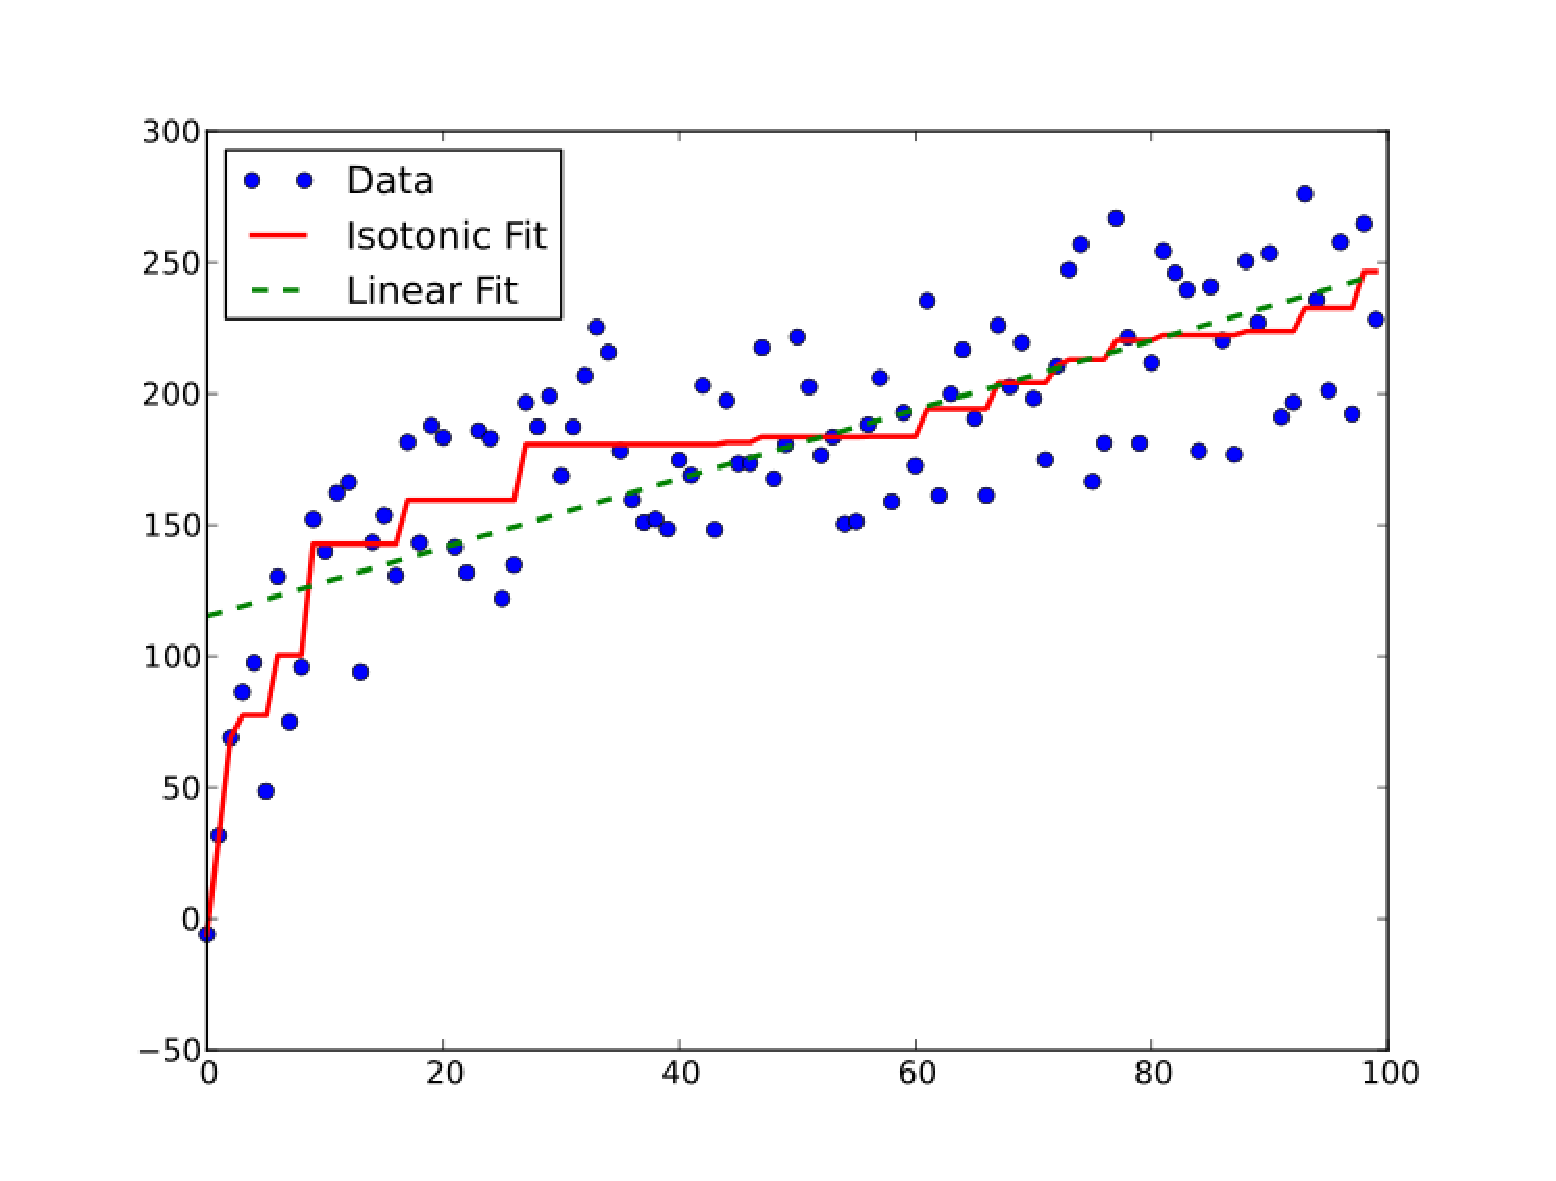
\includegraphics[width=0.7\linewidth]{img/isotonic.eps}
 \caption{Изотоническая регрессия}\label{fig:isotonic}
\end{figure}
\end{center}

Мы хотим найти такую функцию $m(t)$: $P(y = 1 | x) = m(f(x))$. Она настраивается под квадратичную ошибку:

$$m = \argmin_{z} \sum (y_i - z(f(x_i))^2,$$

с помощью специального алгоритма (Pool-Adjacent-Violators Algorithm), изучать который в этом курса не будем.

В результате калибровки получаем надстройку над нашей моделью, которая применяется поверх предсказаний базовой модели. В случае мультиклассовой классификации каждый класс калибруется отдельно против остальных (one-versus-all), вероятности при предсказании нормируются.



\end{document}
